\documentclass{beamer}
\mode<presentation>{
	\usetheme{classic}
	\setbeamercovered{transparent}
	}
\usepackage{hyperref}
\usepackage[T1]{fontenc}

\usepackage[T1]{pbsi} %hand writting nice :P
\usepackage{textcomp} % mai multe:-??

\usepackage{ifpdf}
\usepackage{graphicx}
\usepackage{color}
\usepackage{algorithmic}
\usepackage{algorithm}
\usepackage{amsmath} % formule matematice
\usepackage{palatino, url, multicol} %multicolumns 
\definecolor{lg}{rgb}{0.5,0.5,0.5}

\newcommand{\tbf}{\textbf}
\newcommand{\ds}{\displaystyle}
\newcommand{\ra}{\rightarrow}

\ifpdf
\hypersetup{pdfpagemode=FullScreen}
\fi

\title{\tbf{Dirty money: \\ Feature Selection Using AdaBoost}}
\author{Silvia, Jasper \& Nimrod}
%\subject{bmeps}
\begin{document}

\frame{\titlepage}

%\section[Outline]{}
%\frame{\tableofcontents}

% \beamertemplateshadingbackground{yellow!50}{magenta!50}


\section{Introduction}
	\subsection{Introduction}
	\frame{ 
		\frametitle{Introduction}
		The goal of this project is to be able to distinguish between clean and soiled bills.\\
		\begin{itemize}
		\item bills return to the bank 2 or 3 times a year (1.1 billion bills a year) 
		\item 30\% of 5-\emph{Euro} bills is destroyed
		\item current detection of dirty bills works with reflection of light
		\item best sorting machines destroys 15\% of all bills in order to destroy 95\%
		of the dirty bills
		\item value of good bills that are destroyed in Holland is 1.5 million \emph{Euro} 
		\end{itemize}
		\href{http://www.dnb.nl/binaries/DNBmag208\_tcm46-175321.pdf}{\emph{(DNB Magazine Vol 2, 2008)}}
	}  	

	\subsection{Image data examples}
	\frame{ 
		\frametitle{Image data examples}
		\begin{figure}[H]
			\begin{center}
				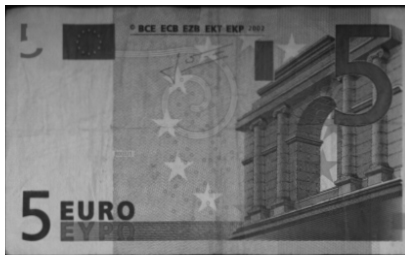
\includegraphics[width=4cm]{img/neur05fit1.jpg}
				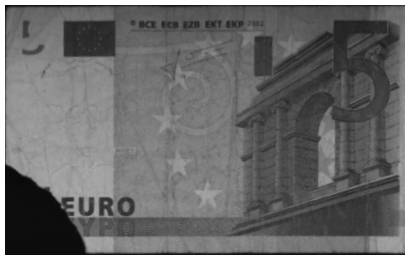
\includegraphics[width=4cm]{img/neur05unfit1.jpg} \\
				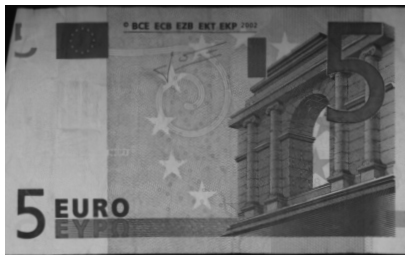
\includegraphics[width=4cm]{img/neur05fit2.jpg}
				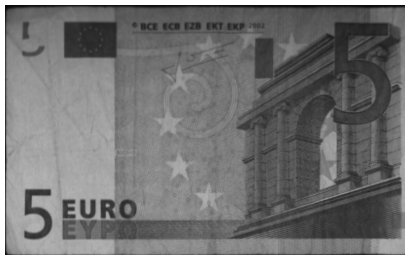
\includegraphics[width=4cm]{img/neur05unfit2.jpg} \\
			\end{center}
			\caption{left: fit bills, right: unfit bills}
		\end{figure}
	}	

\section{Previous work}
	\subsection{DNB Approach}
		\frame{
  			\frametitle{DNB Approach}
  			Uses reflection of light on small area near water mark area.\\
  			\vspace{10pt}\pause
  			Results:
			\begin{itemize}
			\item  5\% dirty bills error 
			\item 30\% clean bills error
			\end{itemize}
  		}
	\subsection{Research by G. Molenaar, A. Nusselder \& K. Stefanov}
		\frame{
  			\frametitle{Research by G. Molenaar, A. Nusselder \& K. Stefanov}
  			Learn Eigen-money using PCA\\
  			\vspace{10pt}\pause
  			Results:
			\begin{itemize}
			\item  \hspace{5px}5 Euro: 12\%  10.5\%  
			\item  10 Euro: 15\% \hspace{2px} 7.5\%  
            \end{itemize} 
  		}
	\subsection{Research by J.M. Geusebroek}
		\frame{
  			\frametitle{Research by J.M. Geusebroek}
  			Pre-processing: 
			\begin{itemize}
				\item bills aligned  
				\item non-linear reflection
				\item water-mark region extracted
            \end{itemize} 
  			Learn Eigen-money on water mark region\\
  			\vspace{10pt}\pause
  			Results:
			\begin{itemize}
			\item  \hspace{5px}5 Euro:  \hspace{7px}3\%  0\% 
			\item  10 Euro: 16\%  6\%  
			\end{itemize}
  		}

\section{Our approach}
\subsection{The task}
		\frame{
			\frametitle{The task}
			Improve classification of 5 and 10 Euro bills and learn some specific features that can be associated with dirt on the bills.\\
			\vspace{10pt}\pause
			We have used \emph{the AdaBoost algorithm} in all methods implemented throughout this project:\\ \pause
			\begin{itemize}
				\item Haar \& convolution
				\item PCA  
				\item Intensity \& edge  
			\end{itemize}\pause
			The algorithm is used to determine the most representative \emph{T} features (the most informative ones).\\
		}

	\subsection{AdaBoost}		
		\frame{
  			\frametitle{AdaBoost algorithm}
			\begin{algorithm}[H] 
				\caption{AdaBoost} 
				\begin{algorithmic}
					\fontfamily{ccr}\selectfont\footnotesize
					\STATE $w_i$ $\leftarrow$ $\left\{\begin{array}{rl}
																\frac{1}{\mid unfit \mid}, & \textcolor{lg}{unfit}$ $\textcolor{lg}{images}\\
																\frac{1}{\mid fit \mid}, & \textcolor{lg}{fit}$ $\textcolor{lg}{images} 
														\end{array}\right.$
					\FOR{t $\leftarrow$ 1 to T} 
						\STATE $w_i$ $\leftarrow$ $\frac{w_i}{\sum_i w_i}$
						\FOR {each feature \emph{j}}
								\STATE \textcolor{lg}{train a weak classifier} \emph{$h_j$} and \textcolor{lg}{compute} $error_j$ $\leftarrow$ $\sum_i w_i \mid h_j(x_i) - y_i\mid$
						\ENDFOR
						\STATE \textcolor{lg}{choose} $h_t$ \textcolor{lg}{which corresponds to} \emph{$min_j(error_j$)}
						\STATE $w_i$	$\leftarrow$ $\left\{\begin{array}{rl}
																w_i \beta_t, & h_t(x_i) = y_i\\
																w_i , & h_t(x_i) \neq y_i
														\end{array}\right.$, \textcolor{lg}{where} $\beta_t = \frac{error_t}{1-error_t}$ 						
					\ENDFOR 
					\STATE \textcolor{lg}{define the strong classifier:}\\
						h(x) $\leftarrow$ $\left\{\begin{array}{rl}
																1, & \sum_t h_t \alpha_t \geq \frac{1}{2} \sum_t \alpha_t\\
																0, & otherwise
														\end{array}\right.$, \textcolor{lg}{where} $\alpha_t = log\frac{1}{\beta_t}$
				\end{algorithmic} 
			\end{algorithm}		
		}


	\subsection{Haar \& convolution}		
		\frame{
  			\frametitle{Haar \& convolution}
			The basic idea of working with \emph{Haar features} is to:\pause
			\begin{itemize}
			\item define a set of patterns of different sizes\pause
			\item loop over the entire image and at each location convolve the corresponding region of image with the patterns\pause	
			\item sum over the resulted values of the pixels for each location, each pattern and each image\pause
			\item use the newly generated values as input features for \emph{AdaBoost} -- \emph{SVM}s are trained for each feature as weak classifiers 
			\end{itemize}
			\begin{figure}[H]
				\begin{center}
					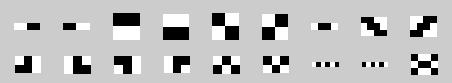
\includegraphics[width=7cm]{img/patterns.jpg}
				\end{center}
			\end{figure}
  		}
		\frame{
  			\frametitle{Haar \& convolution}
			Because the amount of features generated was extremely large we have decided to use only random locations in the image.
				\begin{figure}[H]
					\begin{center}
						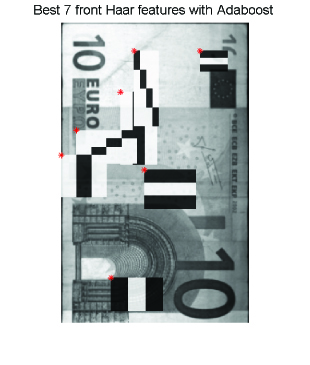
\includegraphics[width=5cm]{img/front_haar.jpg}
						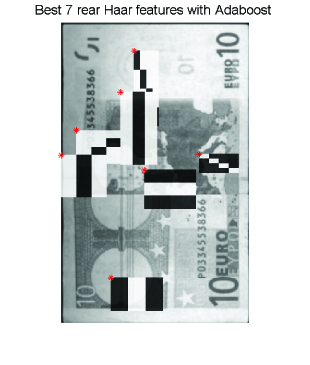
\includegraphics[width=5cm]{img/rear_haar.jpg} \\
					\end{center}
				\end{figure}
		}
		\frame{
  			\frametitle{Haar \& Convolutions}
			New idea:\\
			\begin{itemize}
			\item convolve the entire image with the \emph{Haar patterns} and split the convolved image into overlapping regions\pause
			\item sum over resulted values of the pixels and use these numbers to train weak classifiers in \emph{AdaBoost}\pause 
			\item the weak classifiers are \emph{Gaussians} -- compute the \emph{mean} and \emph{covariance} over all fit/unfit images for each feature (a combination between a pattern and a region)
			\end{itemize}
			\begin{figure}[H]
				\begin{center}
					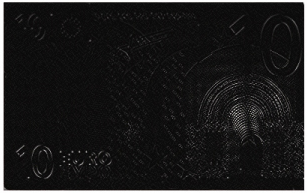
\includegraphics[width=4cm]{img/convolution.jpg} \\			
				\end{center}
			\end{figure}
  		}

	\subsection{PCA \& SVM}		
		\frame{
			\frametitle{PCA \& SVM}
			Idea of using PCA derived from face recognition:
			\begin{itemize}
				\item Reduce dimensionality of the data
				\item Calculate for a set of training examples the best $n$ Eigen-faces
				\item Select a number of Eigen-faces with the biggest variance
				\item Project train- and test-data on the Eigen-faces
			\end{itemize}
			Use \emph{SVM} to create a decision boundary between classes for our classification task
		}
		\frame{
			\frametitle{PCA \& SVM}
			Learning (off-line)
			\begin{itemize}
				\item Divide image data into regions
				\item Extract Eigen-money segments from the regions
				\item Train the \emph{SVM} models using the projected image data
				\item Select best performing models using \emph{AdaBoost}
			\end{itemize}
			\pause
			Classification (on-line)
			\begin{itemize}
				\item Divide incoming image data into regions
				\item Project regions onto the Eigen-money segments 
				\item Predict the class by feeding the \emph{SVM} model the projection
				\item Combine predictions from both front and rear image data with \emph{Naive Bayes}
			\end{itemize}
		}

	\subsection{Intensity \& edge}
		\frame{
			\frametitle{Intensity \& edge}
			Intensity approach is inspired by current approach DNB\\
			\begin{itemize}
				\item Instances are represented as the average intensity of a bill\\
			\end{itemize}
			\vspace{10pt} \pause
			Edge approach is inspired by idea that used bill have more folds
			and wrinkles\\ 
			\begin{itemize}
				\item Instances are represented as the sum of edge-points using a Canny edge filter 
			\end{itemize}
		}

		\frame{
			\frametitle{Intensity \& edge}
				\begin{figure}[H]
					\begin{center}
						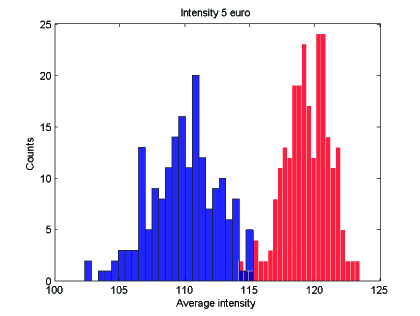
\includegraphics[width=4cm]{img/neur05int.jpg}
						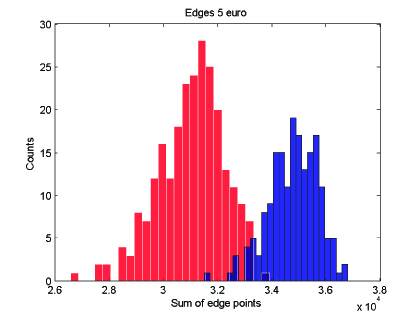
\includegraphics[width=4cm]{img/neur05edge.jpg} \\
						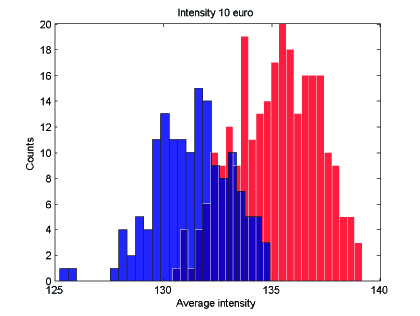
\includegraphics[width=4cm]{img/neur10int.jpg}
						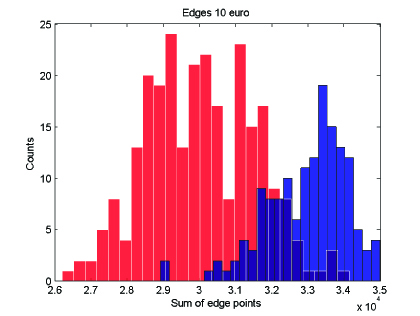
\includegraphics[width=4cm]{img/neur10edge.jpg} \\
					\end{center}
				\end{figure}
		}

		\frame{
			\frametitle{Edges}
			Learning (off-line)
			\begin{itemize}
				\item Perform edge detection on images using Canny edge
				\item Divide edge images into regions and count the edge points
				\item Calculate Gaussian distribution per region over all images
				\item This results in 2 Gaussian distributions (fit and unfit) 
			\end{itemize}
			
			\pause
			Classification (on-line)
			\begin{itemize}
				\item Perform edge detection on incoming image data
				\item Divide edge image into regions and count the edge points
				\item Calculate probability fit and unfit using Gaussian distribution of that region
				\item Classification based on MLE
			\end{itemize}
		}

		\frame{
			\frametitle{Intensity}
			Learning (off-line)
			\begin{itemize}
				\item Divide images into regions
				\item For each region, for each image calculate average intensity
				\item Calculate Gaussian distribution per region over all images
				\item This results in 2 Gaussian distributions (fit and unfit)
			\end{itemize}
			
			\pause
			Classification (on-line)
			\begin{itemize}
				\item Divide edge image into regions
				\item For each region, calculate average intensity
				\item Calculate probability fit and unfit using Gaussian distribution of that region
				\item Classification based on MLE
			\end{itemize}
		}
		
\section{Experiments \& results}

	\subsection{General setup}
	\frame{
		\frametitle{General setup}
		Holdout set:
		\begin{itemize}
			\item $\approx$ 400 images for both 5 and 10 Euro bills
			\item $\approx$ 250 unfit and $\approx$ 150 fit images for both
			\item Extract holdout set of 100 images for both
			\item Develop algorithms and train models on the remaining
		\end{itemize}
		\pause
		Training experiment:
		\begin{itemize}
			\item Split remaining data into train-, test- and validation-set
			\item Perform repeated random sub-sampling validation 
			\item Save best performing model over an arbitrary number of repetitions
		\end{itemize}
	}

	\subsection{Haar Results}
	\frame{
		\frametitle{Results Haar \& Convolution for 5 Euro bills}
		\begin{figure}[H]
			\begin{center}
					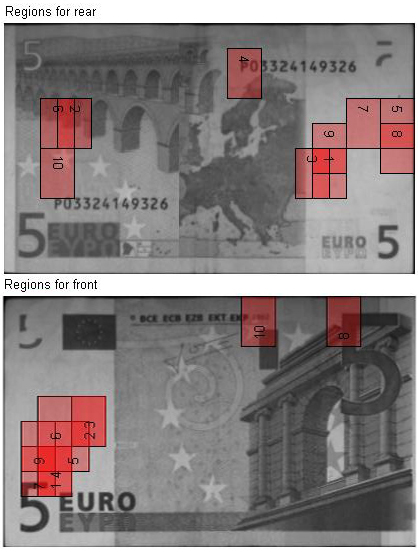
\includegraphics[width=4cm]{img/haar_regions05.jpg}
					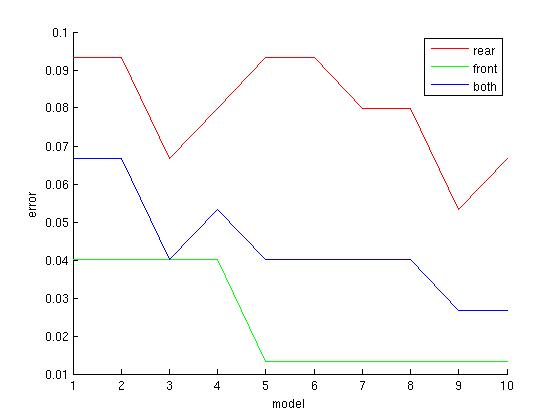
\includegraphics[width=6cm]{img/plot_error05.jpg}
			\end{center}
		\end{figure}						
	}
	\frame{
		\frametitle{Results Haar \& Convolution for 10 Euro bills}
		\begin{figure}[H]
			\begin{center}
					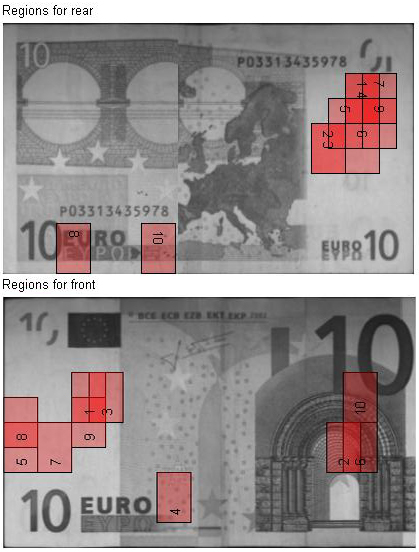
\includegraphics[width=4cm]{img/haar_regions10.jpg}
					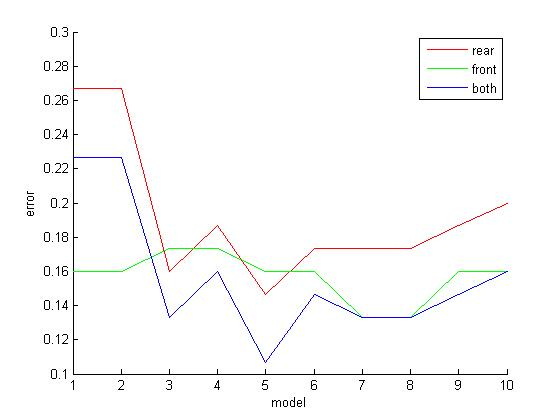
\includegraphics[width=6cm]{img/plot_error10.jpg}
			\end{center}
		\end{figure}				
	}
	\subsection{PCA Results}
	\frame{
		\frametitle{Results PCA -- 5 Euro Bills}
		\begin{figure}[H]
			\begin{center}
					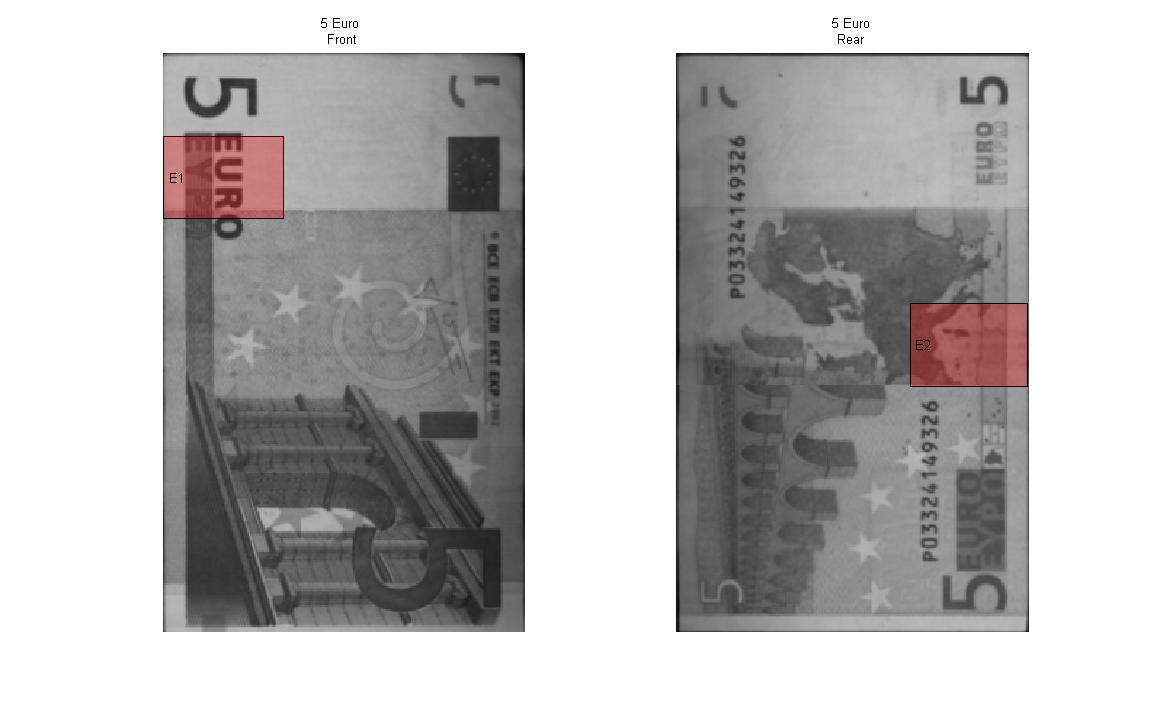
\includegraphics[width=4cm]{img/results_pca_5_regions.jpg}
					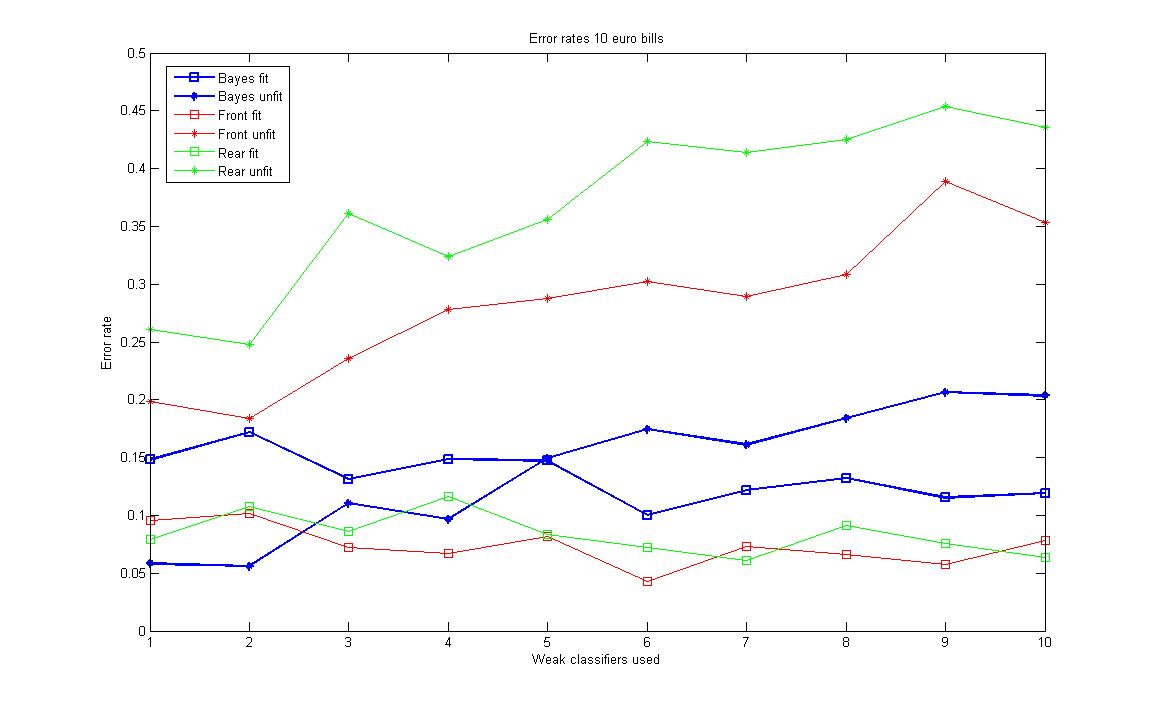
\includegraphics[width=6cm]{img/results_pca_10_plot.jpg}
			\end{center}
		\end{figure}				
	}
	\frame{
		\frametitle{Results PCA -- 10 Euro Bills}
		\begin{figure}[H]
			\begin{center}
					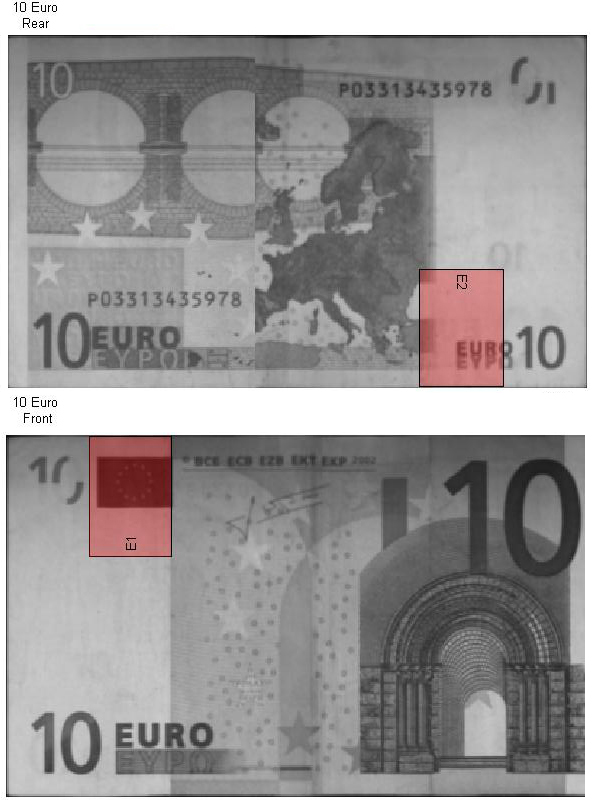
\includegraphics[width=4cm]{img/results_pca_10_regions.jpg}
					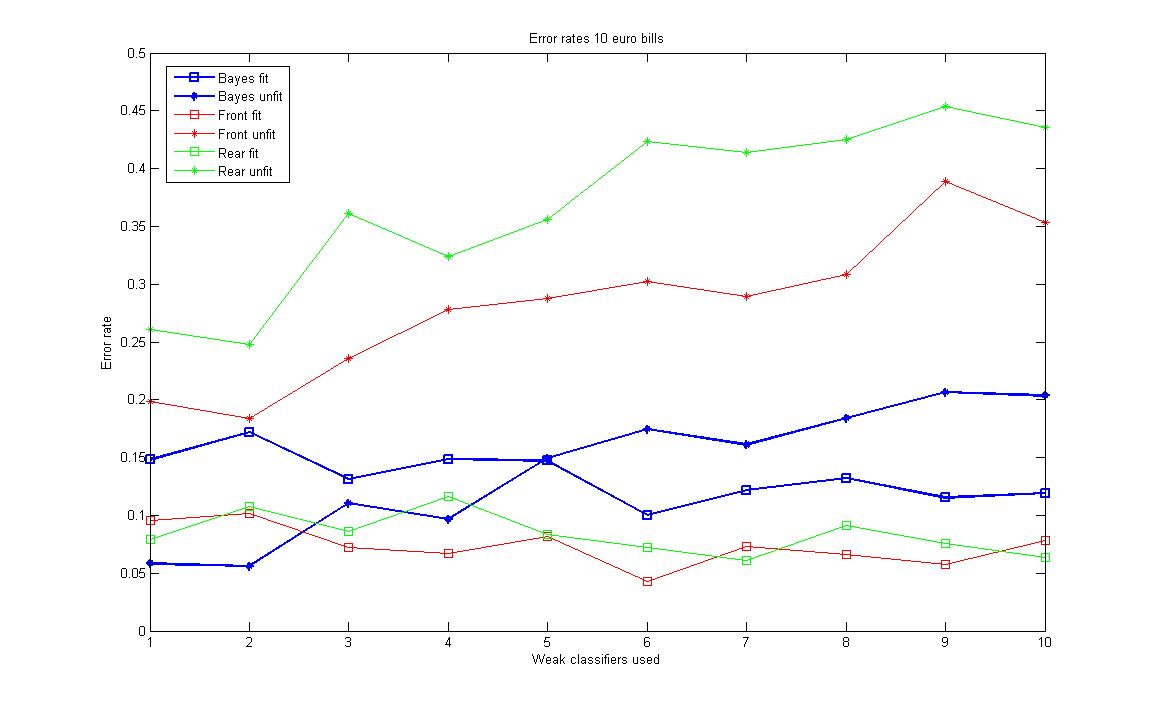
\includegraphics[width=6cm]{img/results_pca_10_plot.jpg}
			\end{center}
		\end{figure}				
	}

	\subsection{Intensity \& Edge Results}
	\frame{
		\frametitle{Results intensity \& edge -- 5 Euro bills} 
		\begin{figure}[H]
			\begin{center}
					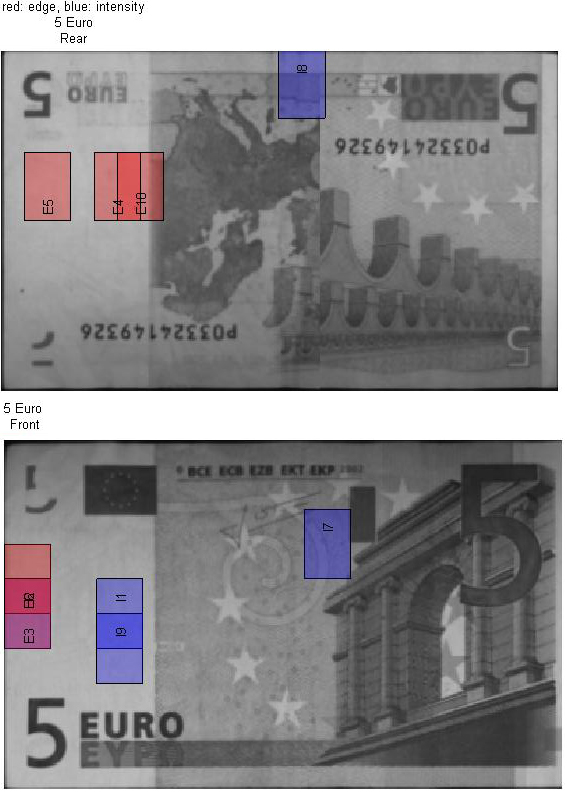
\includegraphics[width=4cm]{img/result_ie_5_regions.jpg}
					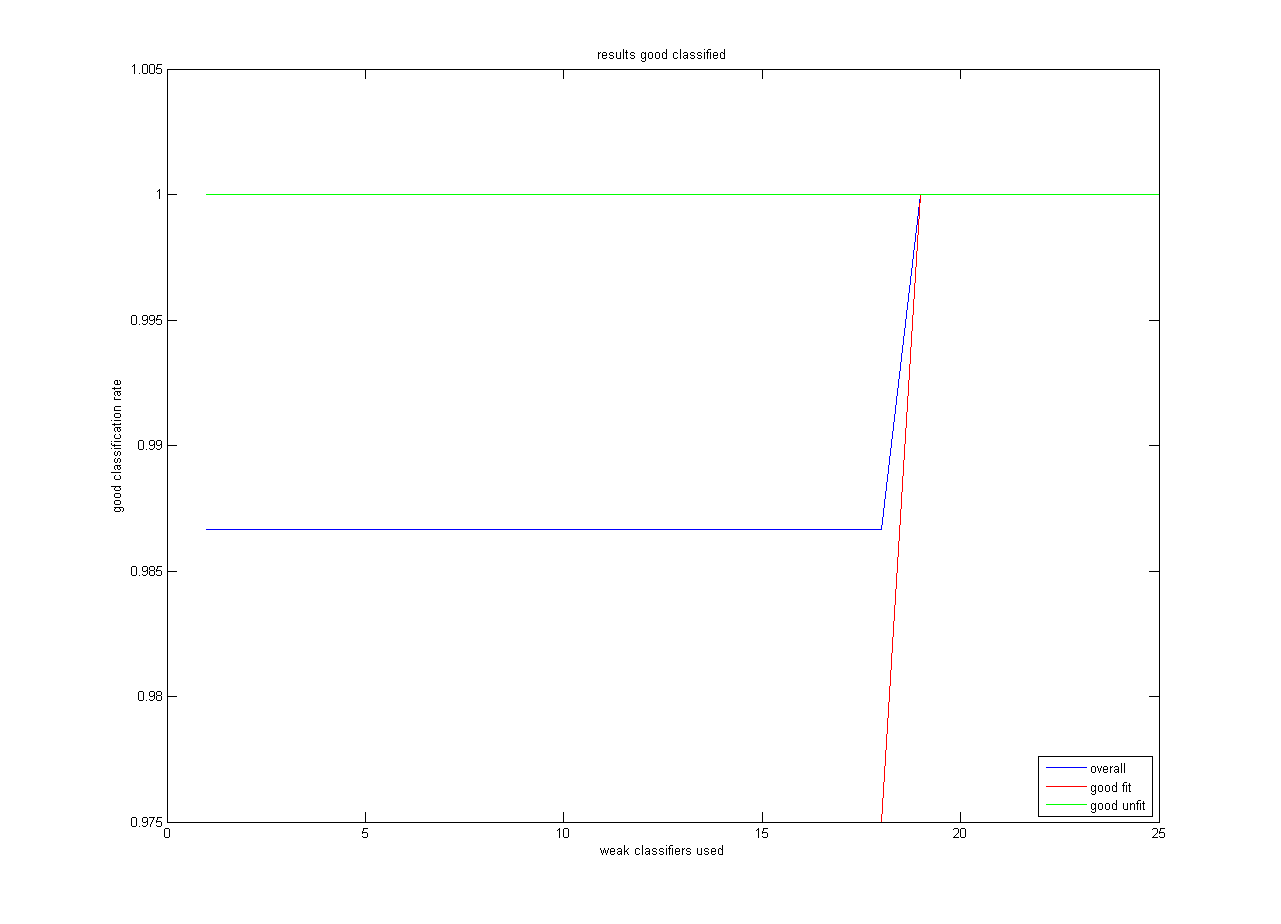
\includegraphics[width=6cm]{img/result_ie_5_plot.png}
			\end{center}
		\end{figure}				
	}
	\frame{
		\frametitle{Results intensity \& edge -- 10 Euro bills}
		\begin{figure}[H]
			\begin{center}
					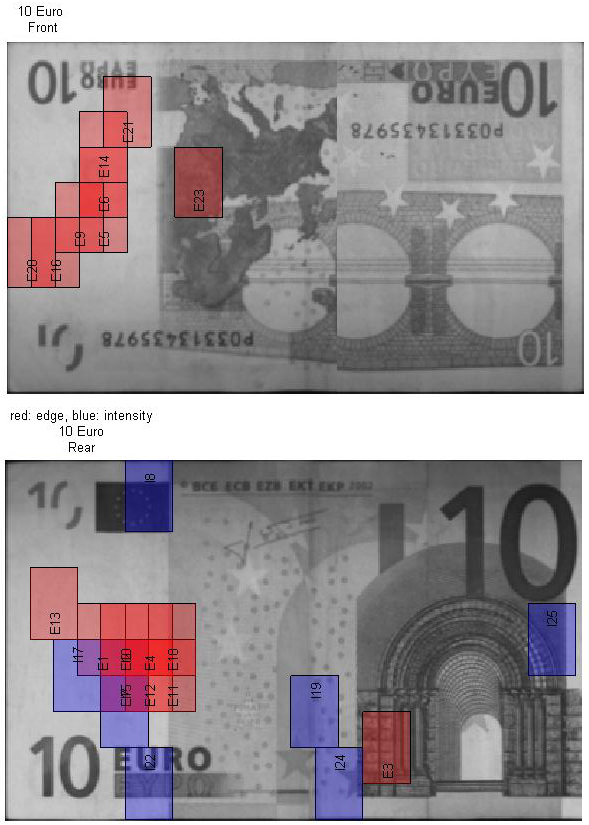
\includegraphics[width=4cm]{img/result_ie_10_regions.jpg}
					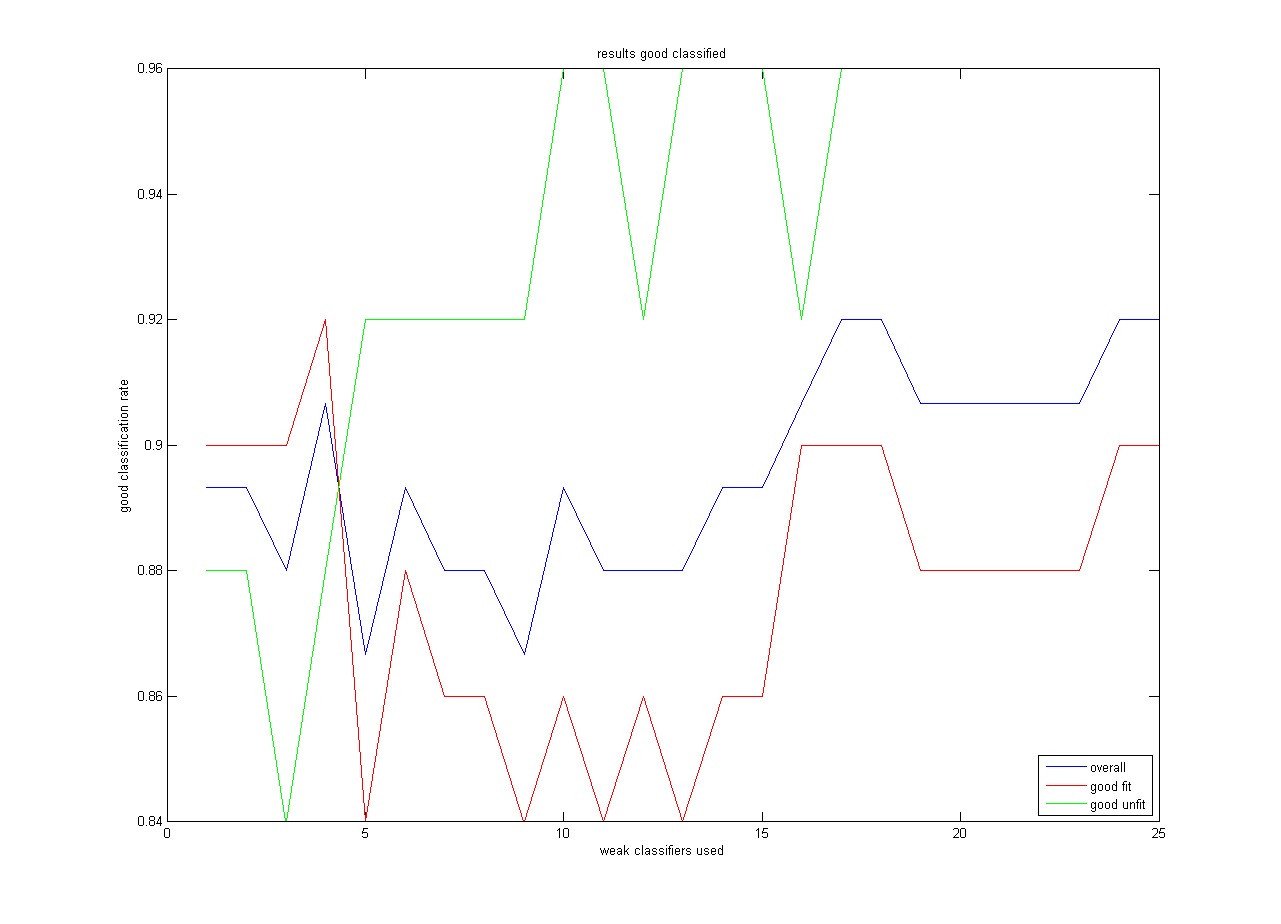
\includegraphics[width=6cm]{img/result_ie_10_plot.png}
			\end{center}
		\end{figure}				
	}

	\subsection{Combined Results}
	\frame{
		\frametitle{Results combined -- 5 Euro Bills}
		\begin{table}[H]
			\caption{Results for 5 Euro Bills}
			\centering 
			\begin{tabular}{ | c | c | c|}
				\hline\hline & \emph{Unfit\break Error} & \emph{Fit\break Error} \\ [0.5ex]\hline 
				\emph{Haar} & 0 & 0 \\ [0.5ex]\hline
				\emph{Intensity - Edge} & 0 & 0.033 \\ [0.5ex]\hline
				\emph{PCA} & 0.025 & 0.083 \\ [0.5ex]\hline
				\emph{Haar \& Intensity - Edge} & 0 & 0 \\ [0.5ex]\hline
				\emph{Haar \& PCA} & 0.025 & 0 \\ [0.5ex]\hline
				\emph{Intensity - Edge \& PCA} & 0.025 & 0.033 \\ [0.5ex]\hline
				\emph{Haar \& Intensity - Edge \& PCA} & 0 & 0.033 \\ [0.5ex]\hline
			\end{tabular}
			\label{table:nonlin} 
		\end{table}		
		}
		
		\subsection{Combined Results}
		\frame{
		\frametitle{Results combined -- 10 Euro Bills}
		\begin{table}[H]
			\caption{Results for 10 Euro Bills}
			\centering 
			\begin{tabular}{ | c | c | c|}
				\hline\hline & \emph{Unfit\break Error} & \emph{Fit\break Error} \\ [0.5ex]\hline 
				\emph{Haar} & 0.15 & 0.05 \\ [0.5ex]\hline
				\emph{Intensity - Edge} & 0.025 & 0.1 \\ [0.5ex]\hline
				\emph{PCA} & 0.05 & 0.083 \\ [0.5ex]\hline
				\emph{Haar \& Intensity - Edge} & 0.15 & 0.033 \\ [0.5ex]\hline
				\emph{Haar \& PCA} & 0.2 & 0.017 \\ [0.5ex]\hline
				\emph{Intensity - Edge \& PCA} & 0.075 & 0.017 \\ [0.5ex]\hline
				\emph{Haar \& Intensity - Edge \& PCA} & 0.025 & 0.033 \\ [0.5ex]\hline
			\end{tabular}
			\label{table:nonlin} 
		\end{table}		
		}

\section{Conclusion}
\subsection{Conclusion}
	\frame{
		\frametitle{Conclusion}
		From our experiments we have learned that:\pause
		\begin{itemize}
		\item The area around the watermark region and the middle of the bills contain the most discriminative features \pause
		\item Combining techniques results in promising performance \pause
		\item Simple methods can outperform more complex methods \pause
		\end{itemize} 
	}

\section{Future work} 
\subsection{Future work}
	\frame{
		\frametitle{Future work}
		For future work we would advise:
		\begin{itemize}
		\item Validate certain features of the images from the data set (intensity)  
		\item Instead of naively combining the strong classifiers (Haar, PCA, Intensity \& Edge) all the features could be combined in \emph{AdaBoost} 
		\end{itemize}
	}
\end{document}

%http://www.dnb.nl/binaries/DNBmag208_tcm46-175321.pdf
